\textbf{Traduce a su correspondiente Modelo Relacional, el problema de la Clínica Veterinaria Si realizaste alguna modificación a tu diseño original (para mejorarlo), indica los cambios hechos y la justificación de éstos. Deberás mostrar el modelo E-R y su correspondiente traducción. Es importante que muestres tanto las restricciones de entidad como las de integridad referencial.}\vspace{.3cm}

Modelo Entidad-Relacion

\begin{center}
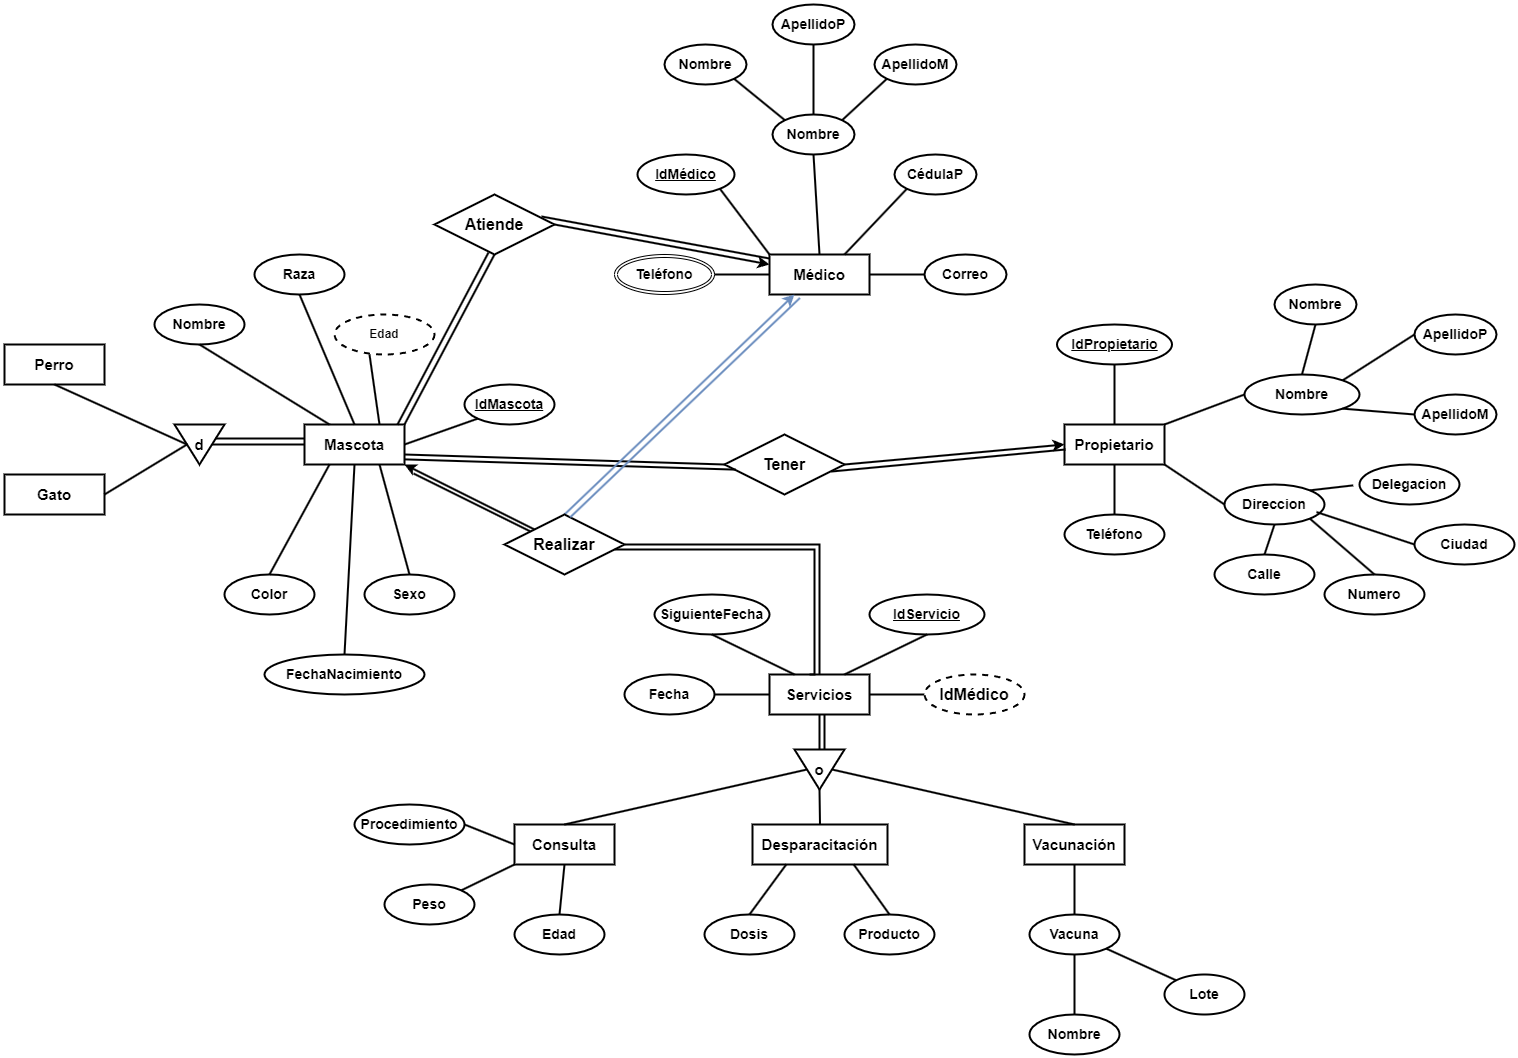
\includegraphics[width=10cm]{resources/Ejercicio3b.png}
\end{center}
Cambios:
\begin{itemize}
    \item En Mascota hemos cambiado la Edad a un atributo calculado
    \item En Servicio cambiamos IdMédico a un atributo calculado
    \item En Propietario cambiamos Teléfono de calculado a normal, ya que en la foto del carnet dado solo se permite un solo teléfono
\end{itemize}

Modelo Relacional

\begin{center}
    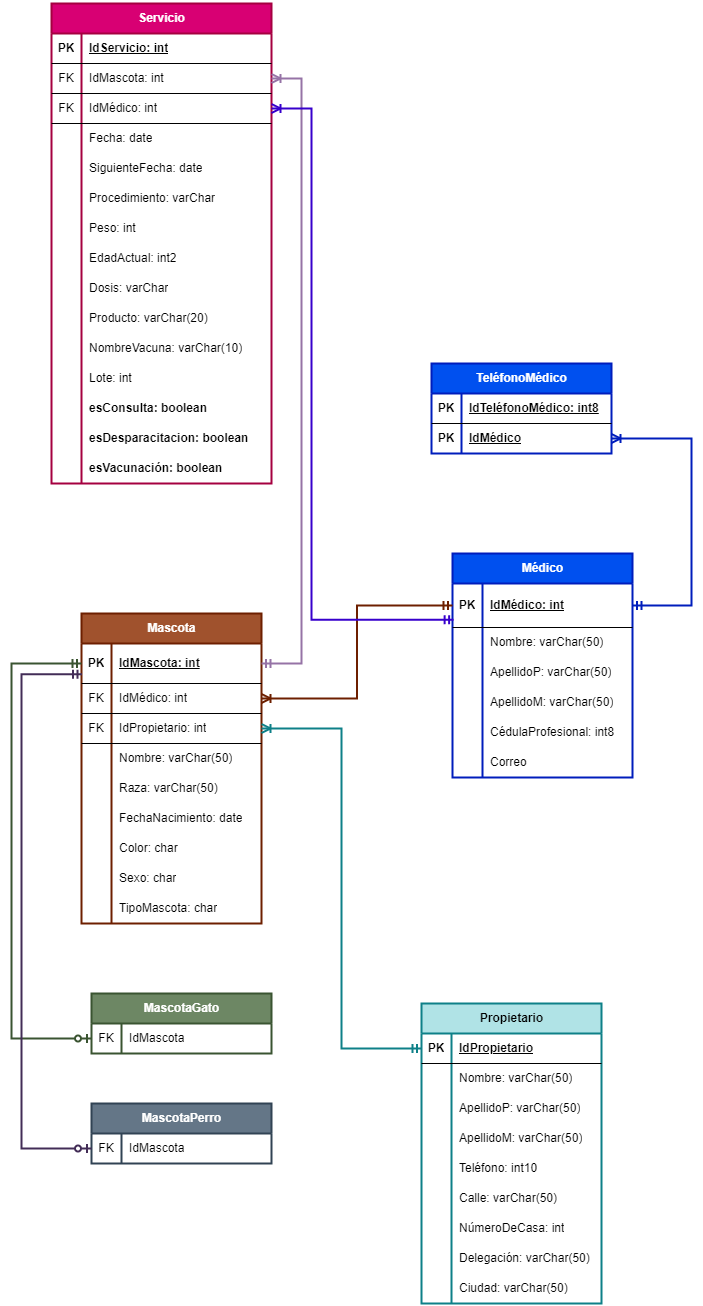
\includegraphics[width=10cm]{resources/Ejercicio2b.png}
    \end{center}

Para Mascota, a pesar de ser herencia disyuntiva obligatoria y no se considera al padre, en este caso decidimos dejarlo para no tener que hacer tantas relaciones para los dos tipos de mascotas que atiende la clínica, esto como el ejemplo de Metro del profe:D 

Claves Foráneas (integridad referencial):

- Servicio: IdMascota referencia a Mascota(IdMascota)

- Servicio: IdMédico referencia a Médico(IdMédico)

- Mascota: IdMédico referencia a Médico(IdMédico)

- Mascota: IdPropietario referencia a Propietario(IdPropietario)

- TeléfonoMédico: IdMédico referencia a Médico(IdMédico)

Estas relaciones aseguran que no se puedan ingresar datos inconsistentes, como un servicio para una mascota que no existe.

- Para esConsulta, esDesparacitacion, esVacunación estos campos solo pueden tener dos estados (verdadero o falso), por lo que boolean es el tipo más apropiado.


- La entidad MascotaGato y MascotaPerro en el modelo relacional es una herencia, lo cual es una buena práctica para manejar atributos específicos de cada tipo de mascota.

